\documentclass[12pt,letterpaper]{exam}

\newcommand{\DocTitle}{Renew the DocTitle variable.}
\newcommand{\CourseNumber}{NE555}
\newcommand{\CourseName}{Nuclear Reactor Dynamics}
\newcommand{\DayTime}{TuTh 8:00-9:15}
\newcommand{\Room}{VV\&E B129}
\newcommand{\Term}{Spring 2011}
\newcommand{\Instructor}{Lewis John Lloyd}
\newcommand{\School}{University of Wisconsin - Madison}

\usepackage{listings}
\usepackage{mathtools}
\usepackage{xtab}
\usepackage{longtable}
\usepackage{array}
\usepackage{mathrsfs}
\usepackage{color}
\usepackage{multicol}
\usepackage{pdflscape}
\usepackage{pdfpages}
\usepackage{graphicx}
\usepackage{esint}
\usepackage{amsmath}
\usepackage{amssymb}
\usepackage{graphics}

\usepackage[
			pdfborder={0 0 0},
			urlcolor=cyan,
			pdftitle={\CourseNumber \DocTitle},
			pdfauthor={\Instructor}
			]{hyperref}
			
\usepackage[
			includeheadfoot,
			top=0.5in,
			bottom=0.5in,
			left=1.0in,
			right=1.0in
			]{geometry}
\setlength{\parindent}{0in}
\setlength{\parskip}{\baselineskip}

\lhead{\CourseNumber: \CourseName}
\chead{}
\rhead{\Term}
\lfoot{}
\cfoot{\thepage}
\rfoot{}
\coverlhead{\CourseNumber: \CourseName}
\coverchead{}
\coverrhead{\Term}
\coverlfoot{}
\covercfoot{\School}
\coverrfoot{}


\correctchoiceemphasis{\bfseries\color{red}}
\bracketedpoints
\pointsinmargin
%\addpoints
%\shadedsolutions

\lstset{ %
language=Matlab,                % the language of the code
basicstyle=\footnotesize,       % the size of the fonts that are used for the code
numbers=left,                   % where to put the line-numbers
numberstyle=\footnotesize,      % the size of the fonts that are used for the line-numbers
stepnumber=5,                   % the step between two line-numbers. If it's 1, each line 
                                % will be numbered
numbersep=5pt,                  % how far the line-numbers are from the code
backgroundcolor=\color{white},  % choose the background color. You must add \usepackage{color}
showspaces=false,               % show spaces adding particular underscores
showstringspaces=false,         % underline spaces within strings
showtabs=false,                 % show tabs within strings adding particular underscores
frame=single,                   % adds a frame around the code
tabsize=2,                      % sets default tabsize to 2 spaces
}

\renewcommand{\solutiontitle}{\noindent\textbf{Solution:}\par\noindent}

\newcommand{\mathsym}[1]{{}}
\newcommand{\unicode}{{}}
\newcommand{\tr}[1]{\tilde{#1}}
\newcommand{\LapTran}[1]{\mathscr{L}\left[#1\right]}
\newcommand{\InvLapTran}[1]{\mathscr{L}^{-1}\left[#1\right]}
\newcommand{\ParDer}[2]{\frac{\partial #1}{\partial #2}}
\newcommand{\Der}[2]{\frac{d\; #1}{d\;#2}}


\renewcommand{\DocTitle}{Problem Set 05}
\noprintanswers

%-------------------------------------------------------------------------------------
\begin{document}
%-------------------------------------------------------------------------------------
\begin{center}
\textbf{\DocTitle}
\end{center}
%-------------------------------------------------------------------------------------
\textbf{NOTES}: 
Use EES for coolant properties.
Show all calculations and \textbf{circle} each requested piece of data.
Answers that are not circled will not be awarded points.
\begin{questions}
%-------------------------------------------------------------------------------------
\question[50]{
A PWR UO$_2$, $k_f$ = 2 [$\frac{W}{m\cdot K}$], fuel pellet has a diameter of 9.3 [mm] and is insulated from the cladding by a helium, $k_{He}$ = 0.25 [$\frac{W}{m\cdot K}$], gas gap. 
The zirconium cladding, $k_c$ = 17 [$\frac{W}{m\cdot K}$], is 0.62 [mm] thick and has an outer diameter of 10.7 [mm].
The fuel pellet experiences slight self-shielding, leading to an internal heat generation given by:
$$q(r)''' = q_o'''\left(1+0.12(\frac{r}{R})^2\right)$$
The average volumetric heat generation in the fuel pellet is 300 [$\frac{MW}{m^3}$].
The fuel rods are arrayed in a square lattice with a pitch-diameter ratio of 1.32.
The coolant, H$_2$O, is flowing past the fuel with a velocity of 2.472 [$\frac{m}{s}$] at 15.5 [MPa] with a bulk temperature of 590 [K].
Use the Dittus-Boelter correlation for forced convection, $Nu = 0.023 Pr^{0.4} Re^{0.8}$, to find the heat transfer coefficient.

What is the algebraic formula for the flow area of the channel in terms of the pitch-diameter ratio and the diameter?

What is the hydraulic diameter of the channel?

What is the mass flow through the channel?

What is the Reynolds Number of the flow?

What is the Nusselt Number of the flow?

What is the heat transfer coefficient?

What is the maximum-average volumetric heat generation ratio in the fuel pellet?

What is the maximum temperature in the fuel?

What is the maximum-average temperature ratio in the fuel pellet?

What is the difference between the average fuel temperature and the cladding outer surface temperature?

\fullwidth{\begin{solution}

\end{solution}}}
\pagebreak
%-------------------------------------------------------------------------------------
\question[50]{
A graphite fuel pebble, $k_f$ = 60 [$\frac{W}{m\cdot K}$], c$_p$ = 710 [$\frac{J}{kg\cdot K}$] ,and $\rho_f$ = 2.267 [$\frac{g}{cm^3}$] , in a PBMR has an outer diameter of 6 [cm].
The uranium containing TRISO particles are uniformly distributed throughout the inner 5 [cm] diameter sphere, yielding a uniform volumetric heat source of 30 [$\frac{MW}{m^3}$].
The pebble is cooled by the forced convection of helium, T$_{bulk}$ = 800 [K], with a heat transfer coefficient of 500 [$\frac{W}{m^2\cdot K}$]. 

Starting from steady state, the power level of the reactor is slowly raised according to the following power transient profile:
$$ \dot{q}'''(t) = \dot{q}'''(0)\cdot(1.5-0.5e^{-0.04\cdot t})$$

Assume that the heat transfer coefficient and coolant bulk temperature remain constant during this transient.

What is the maximum pebble temperature prior to the onset of the transient?

What is the pebble surface temperature prior to the onset of the transient?

What is the average temperature of the pebble prior to the onset of the transient?

What is the Biot number for the pebble?

What is the time constant for the time rate of change of the fuel pebble temperature?

What is the difference between the average pebble temperature and the coolant temperature after 10 seconds?

After 30 seconds?

After 1 minute?

What is the asymptotic temperature difference?

Normalize the time dependent difference in temperature between the pebble average and coolant by the steady state difference and plot this normalized function until its value reaches 95\% of its asymptotic value.

\fullwidth{\begin{solution}

\end{solution}}}
\ifprintanswers
\pagebreak
\fi
%-------------------------------------------------------------------------------------
\end{questions}

\ifprintanswers
\begin{landscape}
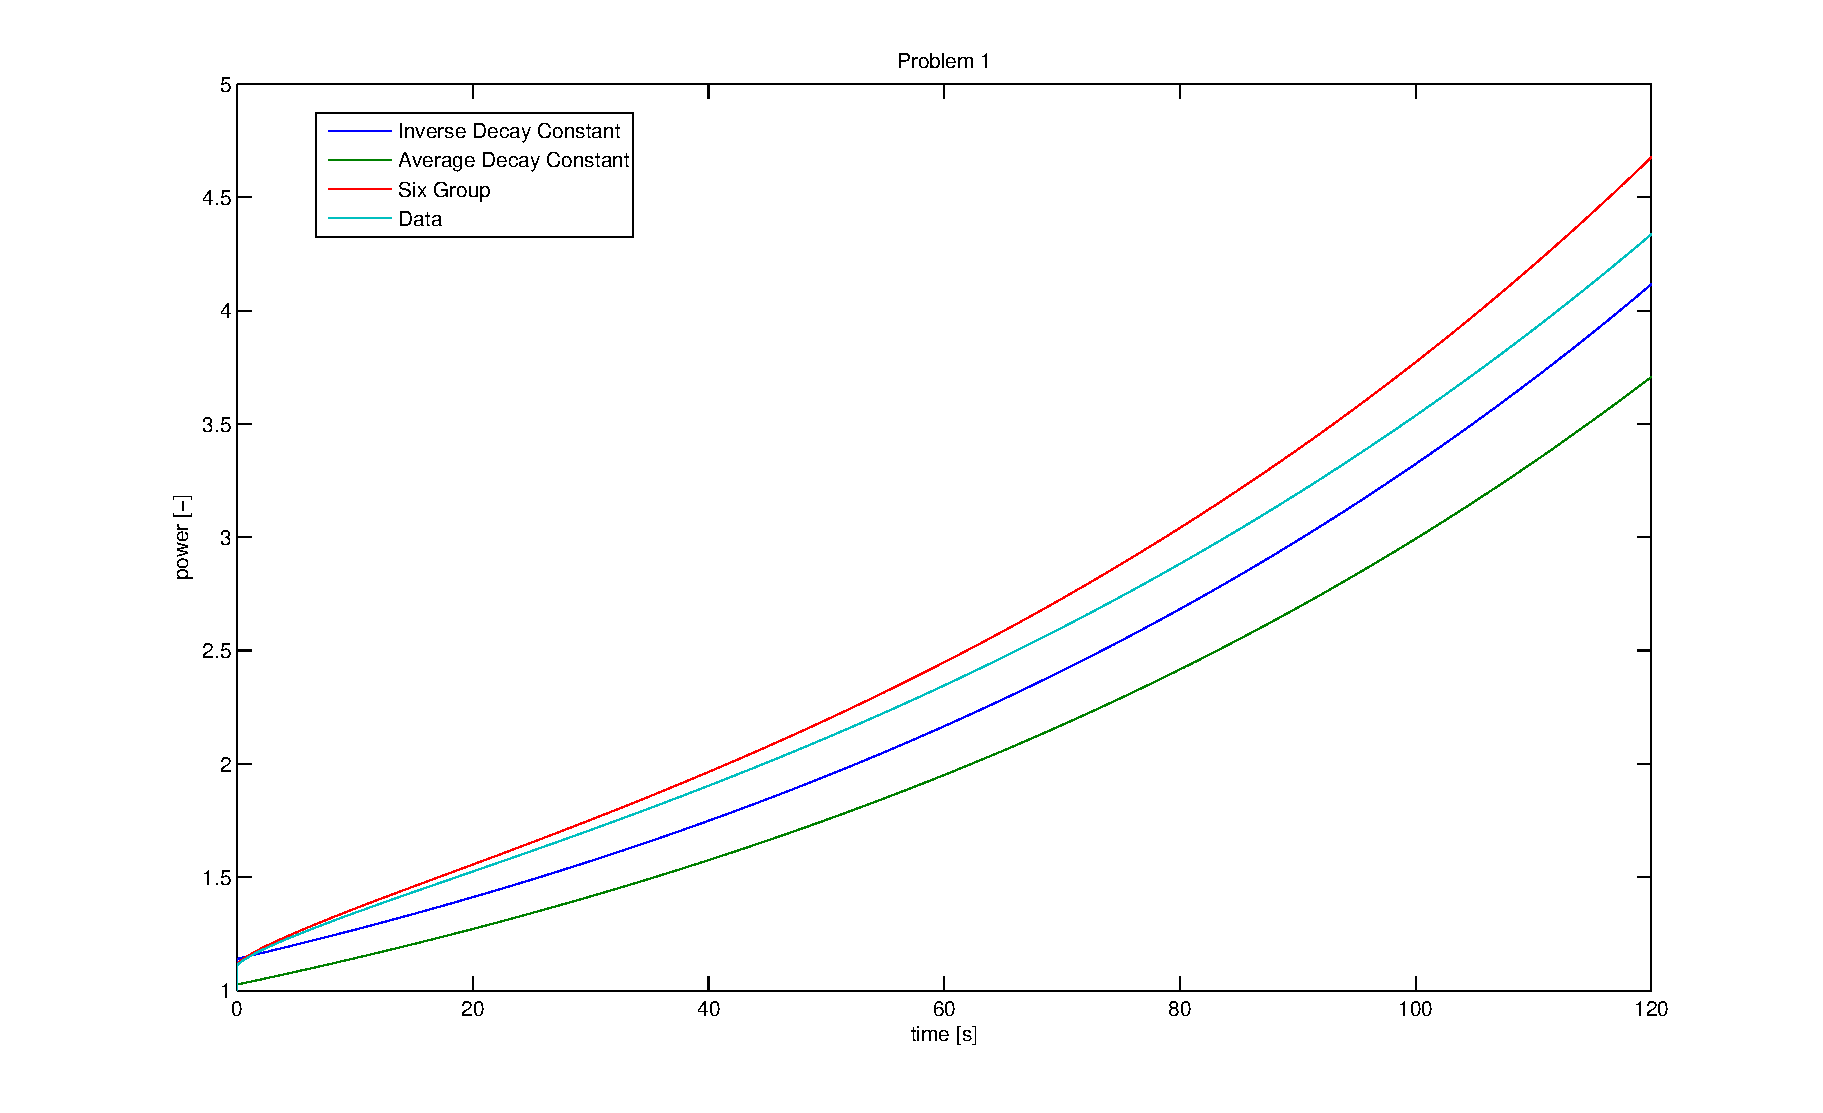
\includepdf[landscape=true]{PS03Q01pic.pdf}
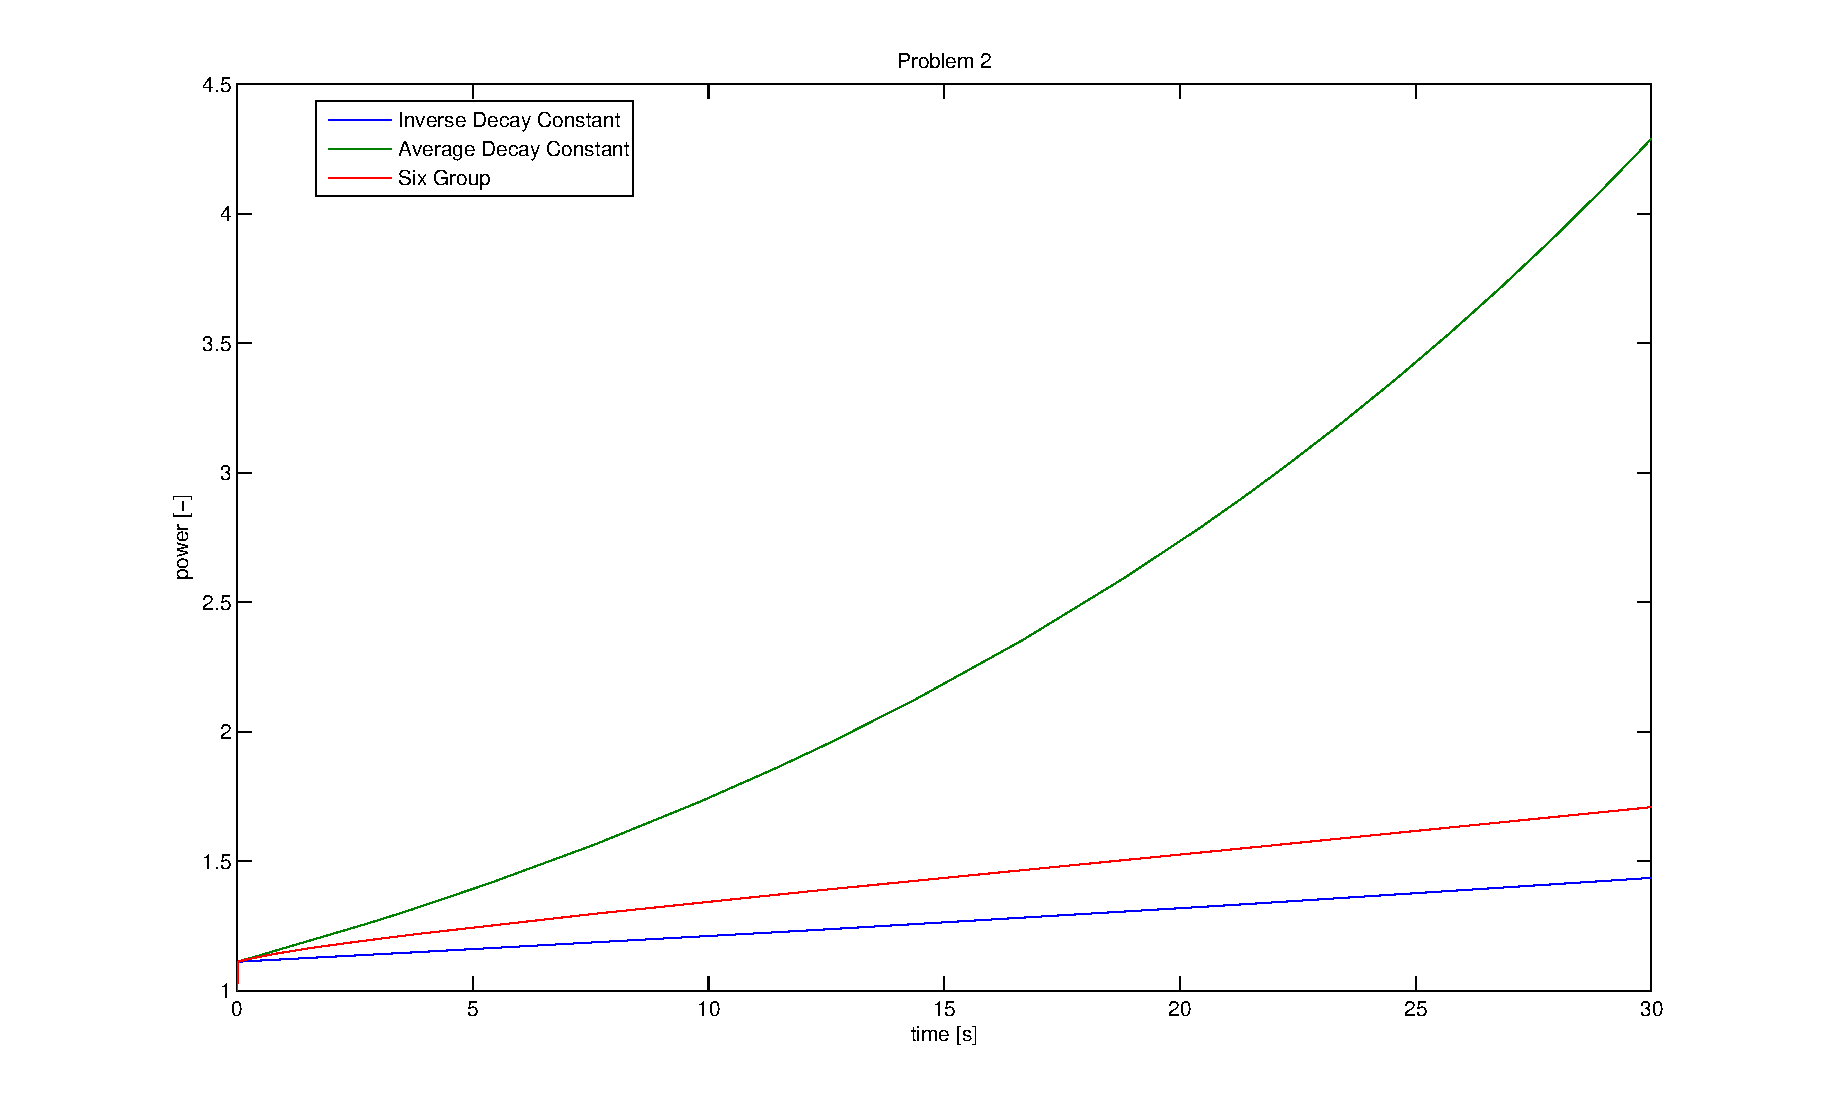
\includepdf[landscape=true]{PS03Q02pic.pdf}
\end{landscape}
\fi

\end{document}